\documentclass{beamer}
% This file is a solution template for:

% - Talk at a conference/colloquium.
% - Talk length is about 20min.
% - Style is ornate.

% Copyright 2004 by Till Tantau <tantau@users.sourceforge.net>.
%
% In principle, this file can be redistributed and/or modified under
% the terms of the GNU Public License, version 2.
%
% However, this file is supposed to be a template to be modified
% for your own needs. For this reason, if you use this file as a
% template and not specifically distribute it as part of a another
% package/program, I grant the extra permission to freely copy and
% modify this file as you see fit and even to delete this copyright
% notice.

%%%%%%%%%%% OPTIONS THAT ARE VALID FOR BOTH HANDOUTS AND NORMAL SLIDES %%%%%%%%
%\usepackage{beamerthemesplit}
\setbeamertemplate{footline}[frame number] % numerar slides
\setbeamertemplate{navigation symbols}{} % retirar barra de navegação

%%%%%%%%%%% OPTIONS THAT ARE VALID FOR NORMAL SLIDES %%%%%%%%
%AK: It seems I do not need it:
%\usepackage{pgfpages}
%\pgfpagesuselayout{resize}[a4paper,border shrink=5mm,landscape]
\mode<presentation> {\usetheme{Singapore}
   \setbeamercovered{transparent}}
   %\mode<presentation> {\usetheme{warsaw} }

   \usepackage[portuguese]{babel}
   \usepackage[utf8]{inputenc}
   %\usepackage[table]{xcolor}
   \usepackage{color}
   \usepackage{booktabs}

   \graphicspath{{../../latex/common_images/},{figures/},{../propor2010/figures/}{figures/telas/}}

   \usepackage{times}
   \usepackage[T1]{fontenc}

\title%[Reconhecimento de Voz para Português Brasileiro] % (optional, use only with long paper titles)
{Transmissor Via Ondas Sonoras}

\author%[]  (optional, for multiple authors)
{Paulo Victor Mocbel \and Pedro Batista \and Tasso Miranda}%\inst{1}}
\institute % (optional)
{
Trabalho Final de Disciplina\\
Análise e Projeto de Sistemas de Software \\
Faculdade de Engenharia de Computação\\
      Universidade Federal do Pará \\
      http://www.laps.ufpa.br/falabrasil\\%\inst{1}
}
% - Use the \inst command only if there are several affiliations.
% - Keep it simple, no one is interested in your street address.

\date[8 de Novembro de 2010] % (optional)
{\today}

%\pgfdeclareimage[height=0.5cm]{university-logo}{figures/logo_laps}
%\logo{\pgfuseimage{university-logo}}
% Delete this, if you do not want the table of contents to pop up at
% the beginning of each subsection:
%\AtBeginSection[]
%{
%  \begin{frame}<beamer>{Sumário}
%  \footnotesize
%     \tableofcontents[currentsection]
%     \end{frame}
%}


% If you wish to uncover everything in a step-wise fashion, uncomment
% the following command:
%\beamerdefaultoverlayspecification{<+->}

\begin{document}

\begin{frame}
\titlepage
\end{frame}

\begin{frame}{Sumário}

\footnotesize
\tableofcontents
% You might wish to add the option [pausesections]
\end{frame}
% Structuring a talk is a difficult task and the following structure
% may not be suitable. Here are some rules that apply for this
% solution:

% - Exactly two or three sections (other than the summary).
% - At *most* three subsections per section.
% - Talk about 30s to 2min per frame. So there should be between about
%   15 and 30 frames, all told.

% - A conference audience is likely to know very little of what you
%   are going to talk about. So *simplify*!
% - In a 20min talk, getting the main ideas across is hard
%   enough. Leave out details, even if it means being less precise than
%   you think necessary.
% - If you omit details that are vital to the proof/implementation,
   %   just say so once. Everybody will be happy with that.

\section{Introdução}

\subsection{Motivação}

\begin{frame}
   \begin{enumerate}
      \item 
      \begin{quote}
	 Mesmo ainda tendo muitos sistemas fazendo uso de fio na transmissão de  dados, o sugimento dos unidades móveis trousse uma nova cara no mercado e com isso a necessidade da comunicação sem fio (wireless).
      \end{quote}
      \item 
	 \begin{quote}
	    Casa Inteligente
	    \begin{figure}[t]

	  \centering

	  \includegraphics[scale=0.35]{casainteligente}

	  \caption{casainteligente}

	  \label{fig:Casa Inteligente}

	  \end{figure}

	 \end{quote}

	 \end{enumerate}

\end{frame}


%-------------------slide02------------------%

\begin{frame}

\subsection{Como?}	

   \begin{enumerate}

      \item {Vantagens:}

	 \begin{quote}

	 \begin{itemize}

	       \item instalação em ambientes de difícil cabeamento;

	       \item centros de distribuição e chão de fábricas;

	       \item empresas em fase de crescimento ou com necessidade constante de reorganização física;

	       \item ambientes que necessitam de montagem rápida e limpa de uma rede local;

	       \item multipercurso.

	 \end{itemize}

	 \end{quote}

      \item Tramissão digital e analógica.

	 \begin{figure}[t]

	 \centering

	 \includegraphics[scale=0.5]{modelo}

	 \caption{modelo}

	 \label{fig:modelo}

	 \end{figure}

      

      \end{enumerate}	      

\end{frame}



%--------------------slide03-----------------%

\begin{frame}

      \begin{enumerate}

	 \item \textit{Modulador} 

	 \begin{quote}

	 \ É responsável pela "adequação" do sinal ao canal que desejamos transporta-lo. No caso do \textit{modulador} digital podemos entende-lo como o mapeador binário, que coloca sinal em forma de ondas apropiadas para transmissão através do canal.

	 \end{quote}

	 \item \textit{Demodulador}

	       \begin{quote}

		  \ Tem a função inversa a do \textit{modulador}, basicamente restabelece o sinal original anteriormente "adequado" ao canal. Tem também a capacidade de detectar ruídos.

	       \end{quote}

      \end{enumerate}

\end{frame}

%---------------slide04---------------%

\begin{frame}

   \begin{enumerate}

      \item \textit{O que ultilizamos?}

	       \begin{itemize}

		  \item filtros passa-faixa,passa-baixas e passa-altas.

		  \item amplificador, transistor.

		  \item {555} 

		     \begin{quote}

			\ É um circuito integrado ultizado em uma variedade de aplicações como temporizador ou multivibrador.

			\begin{figure}[t]

			\centering

			\includegraphics[scale=0.5]{555.png}

			\caption{555}

			\label{fig:555}

			\end{figure}

		     \end{quote}

	       \end{itemize}

   \end{enumerate}

\end{frame}

\section{Embasamento Teórico}
\subsection{Transmissão de Sinais}
\frame{
   \frametitle{Objetivo}
   \begin{itemize}
      \item Levar o sinal.
   \end{itemize}
   \begin{center}
      \includegraphics[height=6cm]{sinal}
   \end{center}
}

\subsection{Modulação e Demodulação AM}

\frame{
   \frametitle{Por que modular?}
   \begin{itemize}
      \item Saber onde sintonizar.
      \item O sinal pode não ser compatível para transmissão.
   \end{itemize}
   \begin{centering}
      \includegraphics[height=3.5cm]{sinal}
      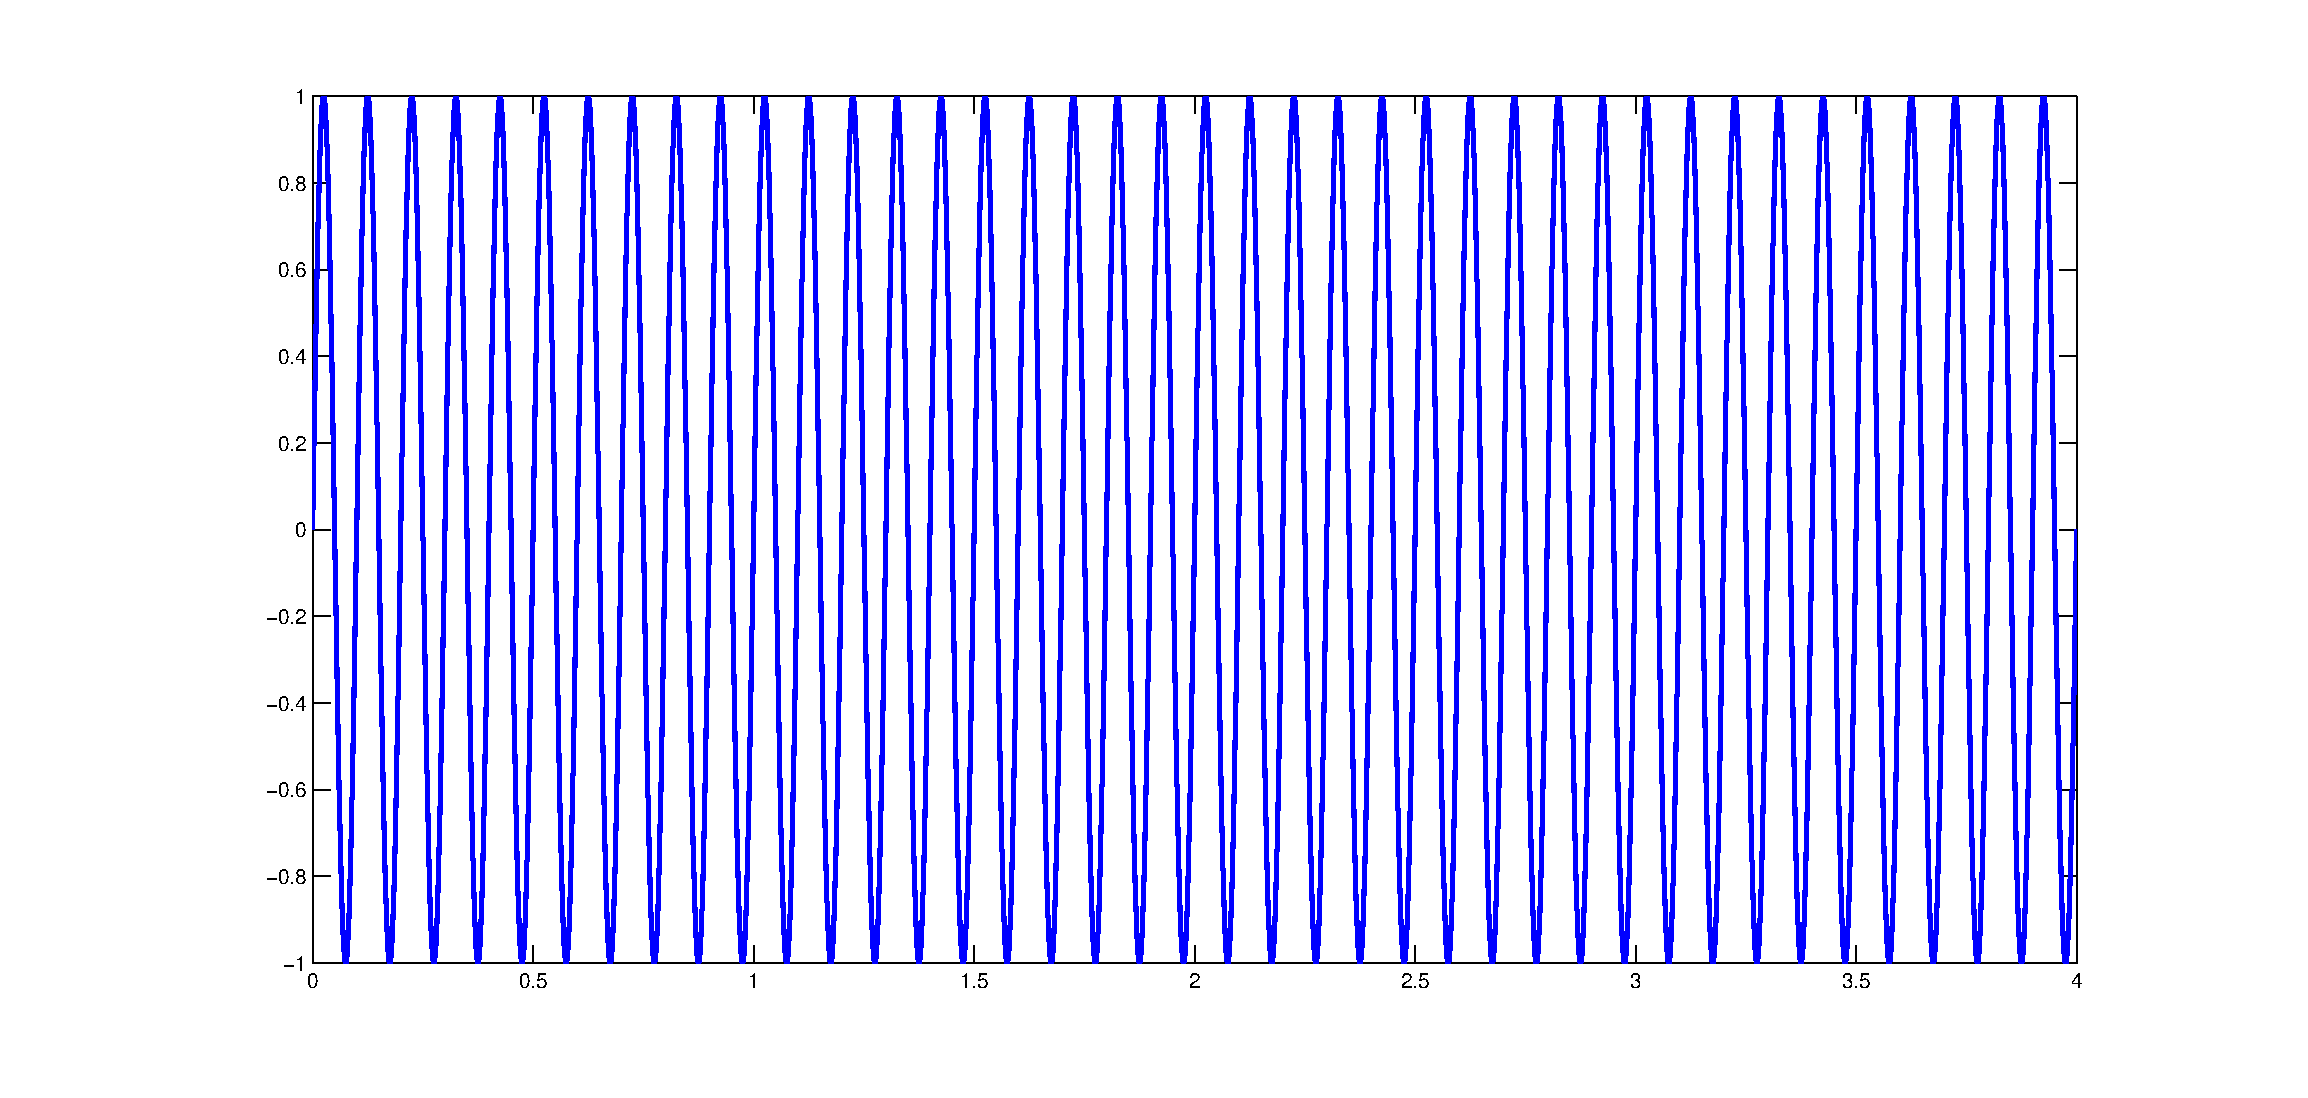
\includegraphics[height=3.5cm]{portadora}
   \end{centering}
}

\frame{
   \frametitle{Modulação AM}
   \begin{centering}
      \includegraphics[height=3.5cm]{sinal}
      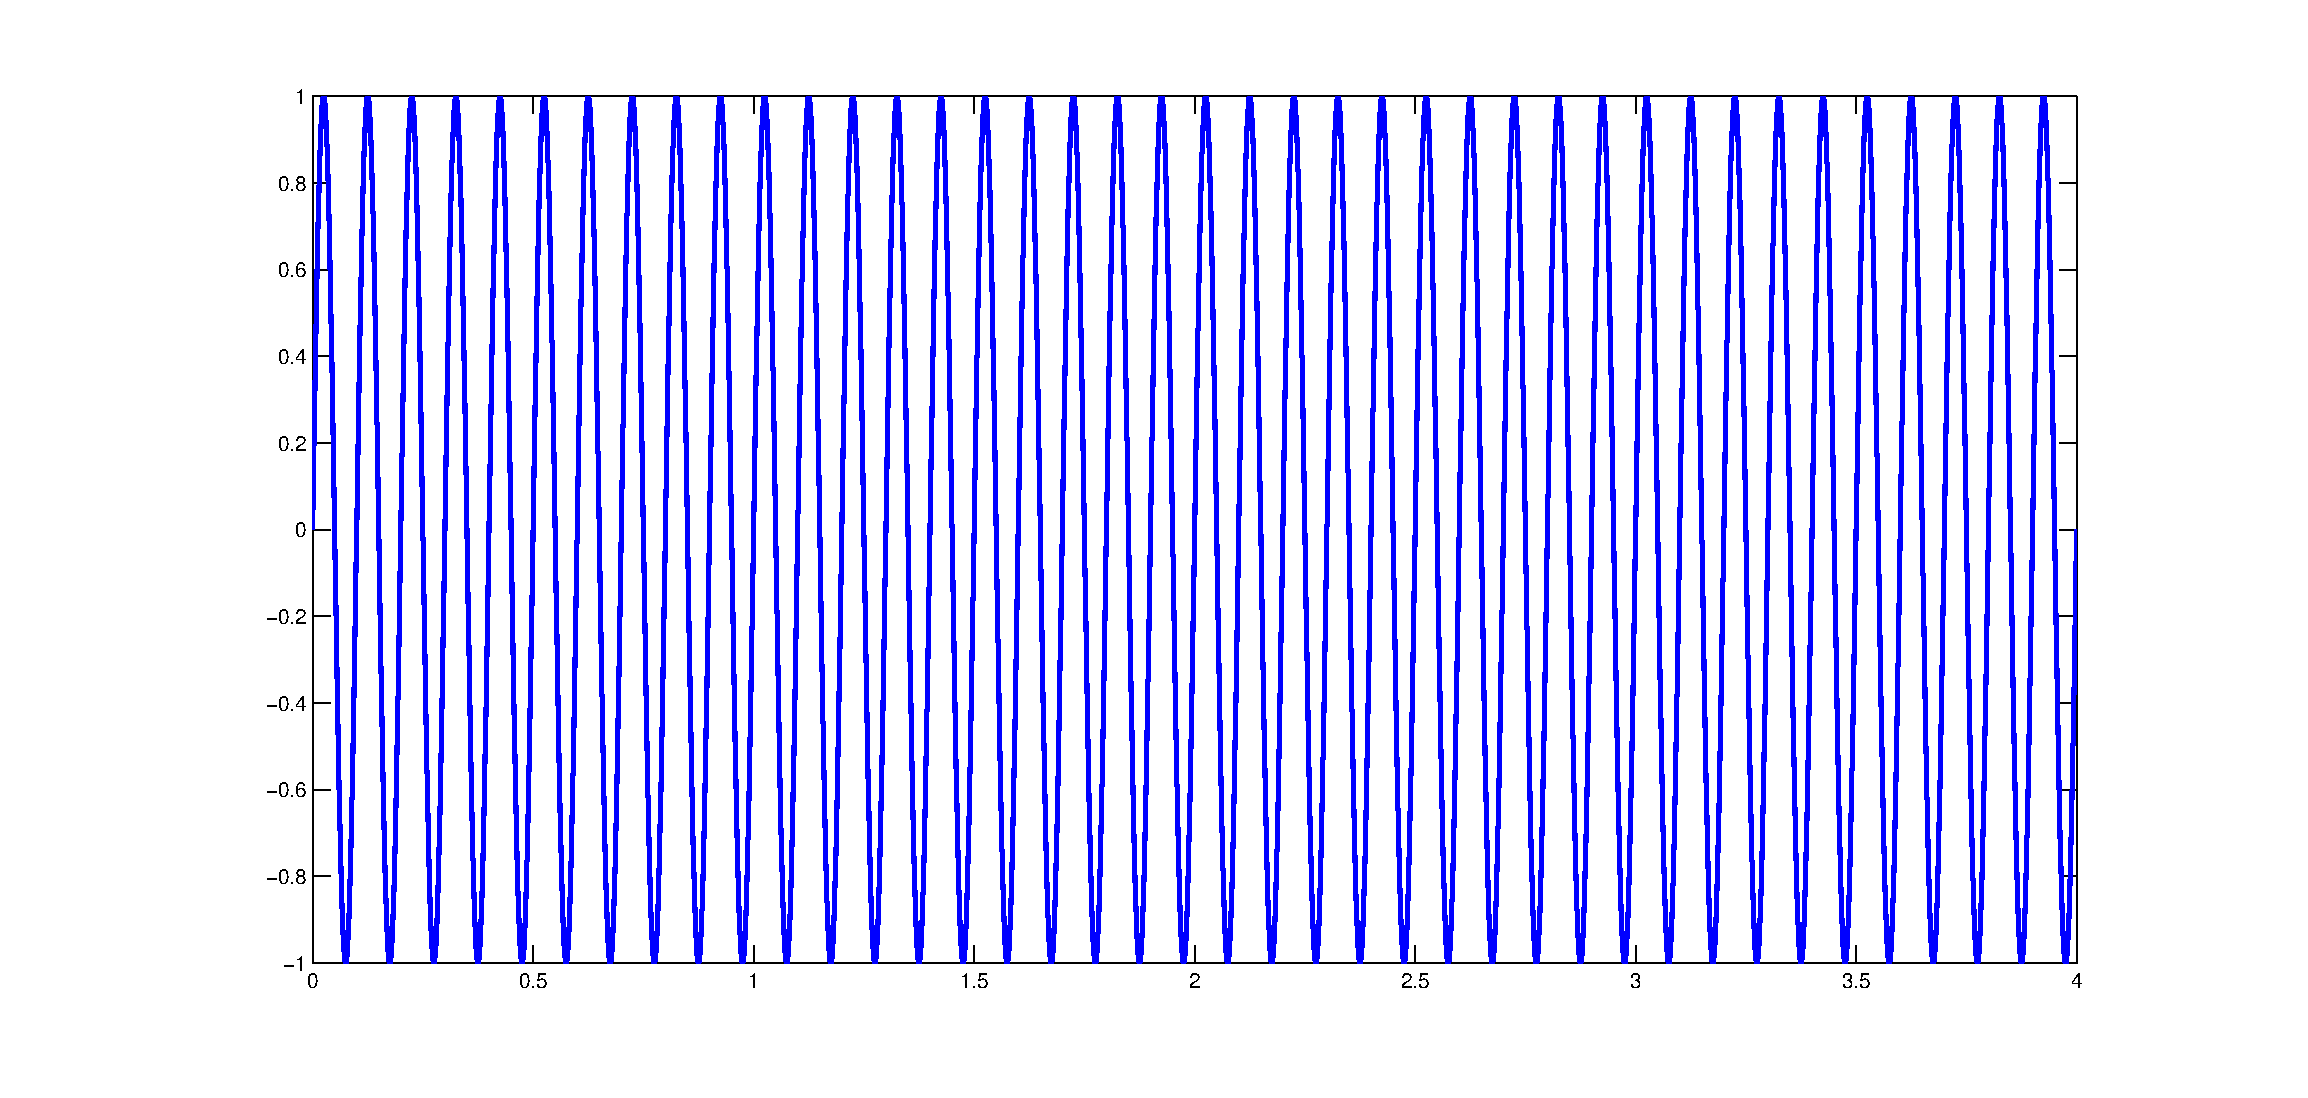
\includegraphics[height=3.5cm]{portadora}\\
      \includegraphics[height=4.5cm]{modulado}
   \end{centering}
}

\frame{
   \frametitle{Recuperação do Sinal - Demodulação}
   \begin{itemize}
      \item Apenas o sinal nos interessa.
   \end{itemize}
   \begin{centering}
      \includegraphics[height=5cm]{modulado}<1>
      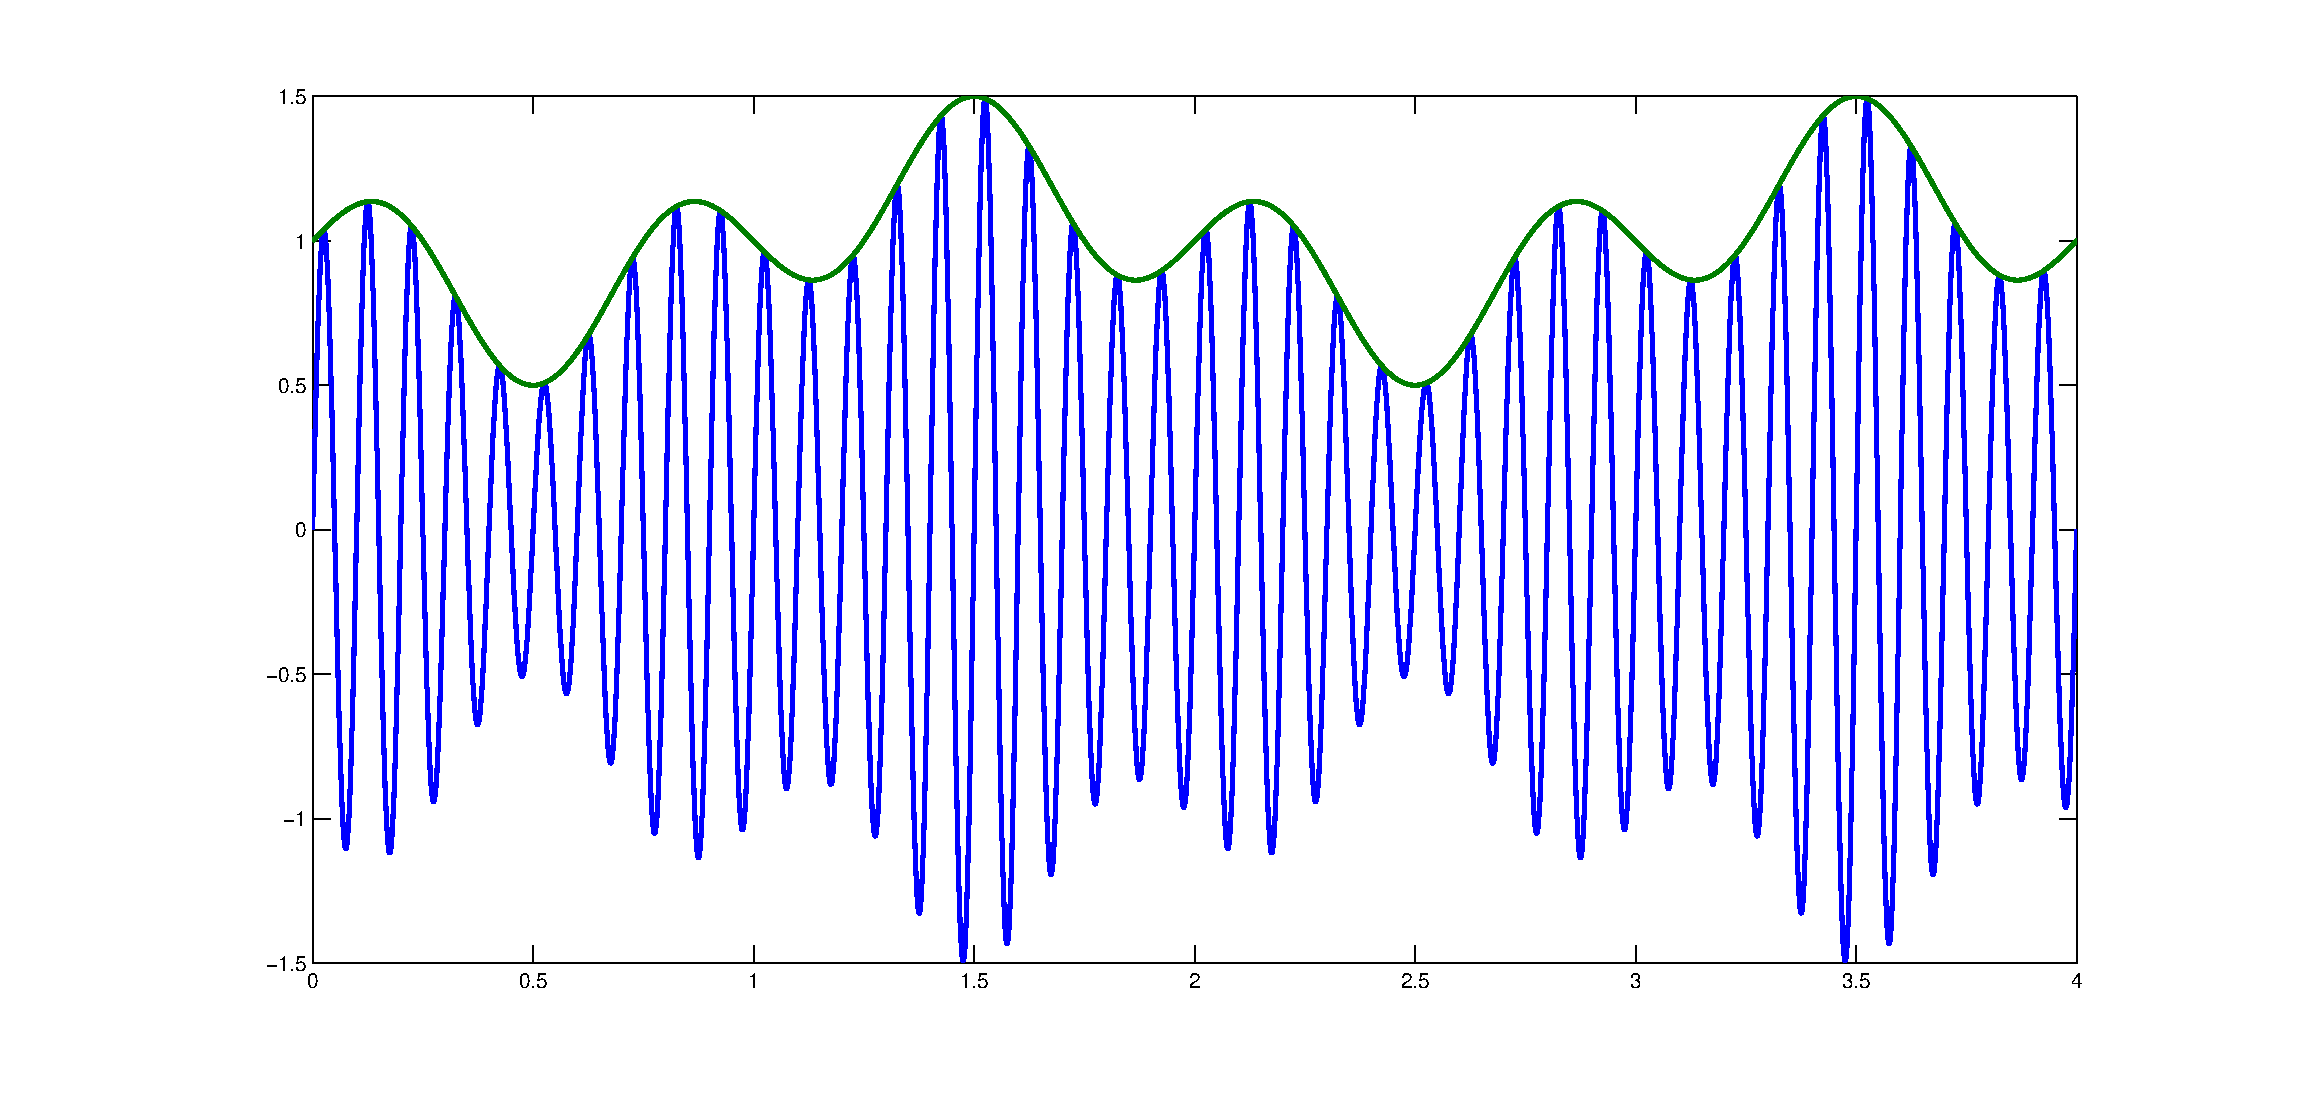
\includegraphics[height=5cm]{modulado_com_sinal}<2>
   \end{centering}
   \begin{itemize}
      \pause
      \item Detector de Envoltória.
   \end{itemize}
}

\subsection{Geração de Ondas o CI 555}

\frame{
   \frametitle{O 555\footnote{Fonte datasheet philips}}
   \begin{itemize}
      \item Features
      \begin{itemize}
	 \item Turn-off time less than 2 us
	 \item Max. operating frequency greater than 500 kHz
	 \item Timing from microseconds to hours
	 \item Operates in both astable and monostable modes
	 \item High output current
	 \item Temperature stability of 0.005 per ºC
      \end{itemize}
   \end{itemize}
   \begin{itemize}
      \item Applications
      \begin{itemize}
	 \item Precision timing
	 \item Pulse generation
	 \item Sequential timing
	 \item Time delay generation
	 \item Pulse width modulation
      \end{itemize}
   \end{itemize}
}

\frame{
   \frametitle{Funcionamento do 555~\footnote{Fonte: Boylestad}}
   \begin{centering}
      \includegraphics[height=3.5cm]{555_interno}
      \includegraphics[height=4cm]{555_configuracao}
   \end{centering}
   \begin{itemize}
      \footnotesize
      \item F/F
      \begin{tabular}{c | c | c}
	 0 & 0 & (estado anterior)\\
	 0 & 1 & 0\\
	 1 & 0 & 1\\
	 1 & 1 & (alterna)\\
      \end{tabular}
   \end{itemize}
}

\frame{
   \frametitle{Slides do tasso}
}

\section{Conclusão}

\frame{
   \frametitle{Conclusão}
   \begin{itemize}
      \item Integração de disciplinas.
      \item Aprendizado de Eletrônica.
      \item Expansão do Circuito.
   \end{itemize}
}

\begin{frame}
   \large
   \frametitle{Obrigado! Perguntas?}
\end{frame}

\end{document}
